Als Vorbereitung der Simulation wurde im Internet nach geeigneten Beispielen zur Simulation von Wasserpumpen gesucht. Dabei sind wir auf das Beispiel ''Well with Jet Pump'' \cite{MathWorks_JetPump} von MathWorks gestossen. Diese Beispielsimulation simuliert einen Brunnenstrahlpumpe, welche sich rund 4.5 Meter im Boden befindet.\\

Da sich bei unserer Simulationsaufgabe die Pumpe jedoch nicht im Boden befinden soll, wurden die entsprechenden Blöcke aus der Schaltung entfernt. Weiter wurden der Wassertankinhalt am Anfang der Simulation auf Null gesetzt. Die erhaltene Schaltung besteht nun aus einem Wassertank, welcher sich auf einer bestimmten Höhe über der Erde befinden kann. Diese ensprechende Höhe des Tankes kann im Pipe-Block entsprechend eingestellt werden. Weiter gibt es eine Zentrifugalpumpe und eine Strahlpumpe, welche sich auf gleichen Niveau, wie die Wasserquelle befindet.\\

Die Zentrifugalpumpe wird wiederrum durch eine mechanische Rotation mit dem Block Velocity Source simuliert. Dieser Block würde man bei einer physischen Umsetzung durch einen DC-Motor ersetzt werden. Damit das Wasser im Becken nicht wieder zurücklaufen kann, wurde ein Check Valve Block verwendet, da dieser nur eine Flussrichtung ermöglicht. Als Flüssigkeit, welche simuliert werden soll, wurde im Water Properties Block, Wasser gewählt.\\

%%%%%%%%%%%%%%%%%%%%%%%%%%%%%%%%%%%%%%%%%%%%%%%%%%%%%%%%%%%%%%%%%%%%%%%%%%%%%
\begin{figure}[htb]
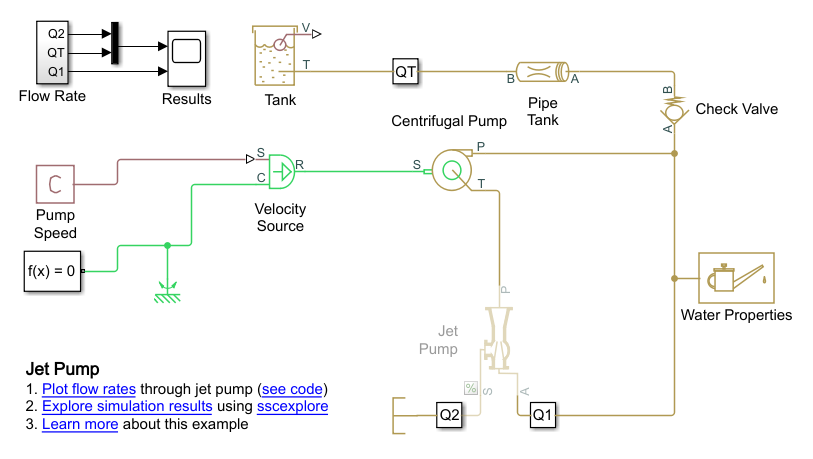
\includegraphics[width=\textwidth]{Simulationsaufbau.png}
\caption{Simulationsaufbau in MATLAB Simulink}
\label{fig:Simulationsaufbau in MATLAB Simulink}
\end{figure}
%%%%%%%%%%%%%%%%%%%%%%%%%%%%%%%%%%%%%%%%%%%%%%%%%%%%%%%%%%%%%%%%%%%%%%%%%%%%%

Die in Abbildung \ref{fig:Simulationsaufbau in MATLAB Simulink} ersichtliche Schaltung zeigt das Ergebnis mit den schliesslich die Simulationen gemacht wurden. Simuliert wurden die einzelnen Fliessraten der Strahlpumpe, sowie das Wasservolumen im Wassertank. Diese Simulation wurde dann schliesslich 10 Sekunden lang simuliert.